\apendice{Especificación de Requisitos}

\section{Introducción}
Una muestra de cómo podría ser una tabla de casos de uso:


\section{Objetivos generales}
El objetivo de este proyecto es desarrollar una aplicación web para poder llevar a cabo la gestión de los departamentos de la Universidad de Burgos. El sistema gestionará el profesorado, asignaturas, reconocimiento de docencia...

\section{Catalogo de requisitos}
A continuación se van a exponer los requisitos de la aplicación web.

\begin{itemize}
	\item \textbf{RF-01.} Se deben diferenciar los roles de administrador y profesor.
	\item \textbf{RF-02.} Mantenimiento de titulaciones.
	\item \textbf{RF-03.} Mantenimiento de asignaturas.
	\item \textbf{RF-04.} Mantenimiento de grupos de asignaturas.
	\item \textbf{RF-05.} Mantenimiento de docentes.
	\item \textbf{RF-06.} Mantenimiento de centros.
	\item \textbf{RF-07.} Un administrador puede asignar horas a un docente en un grupo.
	\item \textbf{RF-08.} Un profesor puede obtener información acerca de los grupos que tiene asignados.
	\item \textbf{RF-09.} Un profesor puede modificar sus datos.
\end{itemize}

\section{Especificación de requisitos}
\subsection{Casos de uso}
% Comando para insertar una imagen en un lugar concreto.
% Los parámetros son:
% 1 --> Ruta absoluta/relativa de la figura
% 2 --> Texto a pie de figura
% 3 --> Tamaño en tanto por uno relativo al ancho de página
\begin{figure}[!h]
	\centering
	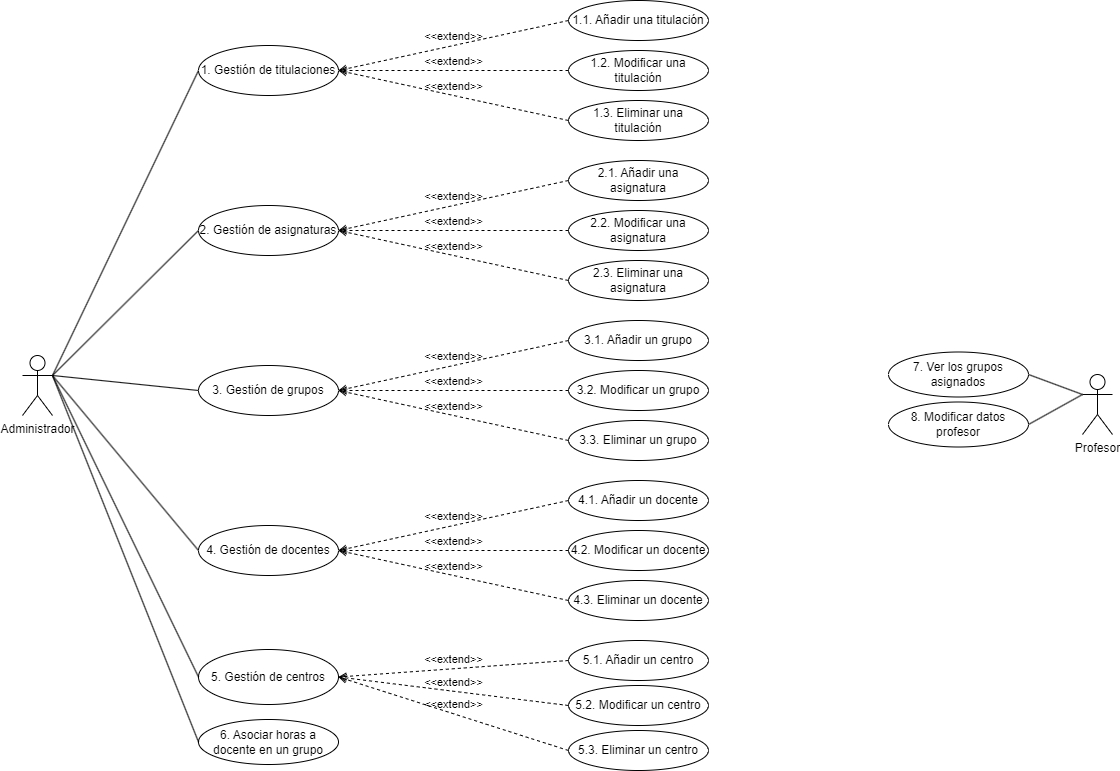
\includegraphics[width=\textwidth]{../img/Anexos/Casos de uso.png}
	\caption{Diagrama de casos de uso}\label{fig:../img/Anexos/Casos de uso.png}
\end{figure}
\FloatBarrier

\begin{table}[p]
	\centering
	\begin{tabularx}{\linewidth}{ p{0.21\columnwidth} p{0.71\columnwidth} }
		\toprule
		\textbf{CU-1.1}    & \textbf{Añadir una titulación}\\
		\toprule
		\textbf{Versión}              & 1.0    \\
		\textbf{Autor}                & Ignacio Dávila García \\
		\textbf{Requisitos asociados} & RF-01, RF-02 \\
		\textbf{Descripción}          & Un usuario administrador añade una nueva titulación \\
		\textbf{Precondición}         & Tener iniciada sesión con una cuenta con permisos de administración \\
		\textbf{Acciones}             &
		\begin{enumerate}
			\def\labelenumi{\arabic{enumi}.}
			\tightlist
			\item Pulsar en la opción titulaciones del menú superior de la web.
			\item Se abre una ventana donde aparece una tabla con las titulaciones creadas.
			\item Pulsar sobre el botón nuevo
			\item Se abre una nueva ventana con un formulario.
			\item Rellenar el formulario con los datos de la titulación que se desea añadir.
			\item Pulsar sobre el botón añadir.
		\end{enumerate}\\
		\textbf{Postcondición}        & El sistema lleva al usuario a la ventana de titulaciones donde se puede ver el listado de todas las titulaciones creadas. \\
		\textbf{Excepciones}          & Se dejan campos vacíos o se introducen datos con un formato incorrecto \\
		\textbf{Importancia}          & Alta \\
		\bottomrule
	\end{tabularx}
	\caption{CU-1.1 Añadir una titulación.}
\end{table}

\begin{table}[p]
	\centering
	\begin{tabularx}{\linewidth}{ p{0.21\columnwidth} p{0.71\columnwidth} }
		\toprule
		\textbf{CU-1.2}    & \textbf{Modificar una titulación}\\
		\toprule
		\textbf{Versión}              & 1.0    \\
		\textbf{Autor}                & Ignacio Dávila García \\
		\textbf{Requisitos asociados} & RF-01, RF-02 \\
		\textbf{Descripción}          & Un usuario administrador modifica una titulación \\
		\textbf{Precondición}         & Tener iniciada sesión con una cuenta con permisos de administración \\
		\textbf{Acciones}             &
		\begin{enumerate}
			\def\labelenumi{\arabic{enumi}.}
			\tightlist
			\item Pulsar en la opción titulaciones del menú superior de la web.
			\item Se abre una ventana donde aparece una tabla con las titulaciones creadas.
			\item Pulsar sobre el botón modificar de la titulación que se desea modificar.
			\item Se abre una nueva ventana con un formulario que tiene los campos rellenos con los datos de esa titulación.
			\item Modificar los campos que se desean cambiar.
			\item Pulsar sobre el botón modificar.
		\end{enumerate}\\
		\textbf{Postcondición}        & El sistema lleva al usuario a la ventana de titulaciones donde se puede ver el listado de todas las titulaciones creadas. \\
		\textbf{Excepciones}          & Se dejan campos vacíos o se introducen datos con un formato incorrecto \\
		\textbf{Importancia}          & Alta \\
		\bottomrule
	\end{tabularx}
	\caption{CU-1.2 Modificar una titulación.}
\end{table}

\begin{table}[p]
	\centering
	\begin{tabularx}{\linewidth}{ p{0.21\columnwidth} p{0.71\columnwidth} }
		\toprule
		\textbf{CU-1.3}    & \textbf{Eliminar una titulación}\\
		\toprule
		\textbf{Versión}              & 1.0    \\
		\textbf{Autor}                & Ignacio Dávila García \\
		\textbf{Requisitos asociados} & RF-01, RF-02 \\
		\textbf{Descripción}          & Un usuario administrador elimina una titulación \\
		\textbf{Precondición}         & Tener iniciada sesión con una cuenta con permisos de administración \\
		\textbf{Acciones}             &
		\begin{enumerate}
			\def\labelenumi{\arabic{enumi}.}
			\tightlist
			\item Pulsar en la opción titulaciones del menú superior de la web.
			\item Se abre una ventana donde aparece una tabla con las titulaciones creadas.
			\item Pulsar sobre el botón eliminar de la titulación que se desea dar de baja.
			\item Se abre una ventana flotante donde se pregunta si está seguro de eliminar la titulación.
			\item Pulsar sobre el botón si.
		\end{enumerate}\\
		\textbf{Postcondición}        & El sistema lleva al usuario a la ventana de titulaciones donde se puede ver el listado de todas las titulaciones creadas. \\
		\textbf{Excepciones}          & Se intenta eliminar una titulación que está vinculada a alguna asignatura \\
		\textbf{Importancia}          & Alta \\
		\bottomrule
	\end{tabularx}
	\caption{CU-1.3 Eliminar una titulación.}
\end{table}

\begin{table}[p]
	\centering
	\begin{tabularx}{\linewidth}{ p{0.21\columnwidth} p{0.71\columnwidth} }
		\toprule
		\textbf{CU-2.1}    & \textbf{Añadir una asignatura}\\
		\toprule
		\textbf{Versión}              & 1.0    \\
		\textbf{Autor}                & Ignacio Dávila García \\
		\textbf{Requisitos asociados} & RF-01, RF-03 \\
		\textbf{Descripción}          & Un usuario administrador añade una nueva asignatura \\
		\textbf{Precondición}         & Tener iniciada sesión con una cuenta con permisos de administración \\
		\textbf{Acciones}             &
		\begin{enumerate}
			\def\labelenumi{\arabic{enumi}.}
			\tightlist
			\item Pulsar en la opción asignaturas del menú superior de la web.
			\item Se abre una ventana donde aparece una tabla con las asignaturas creadas.
			\item Pulsar sobre el botón nuevo
			\item Se abre una nueva ventana con un formulario.
			\item Rellenar el formulario con los datos de la asignaturas que se desea añadir.
			\item Pulsar sobre el botón añadir.
		\end{enumerate}\\
		\textbf{Postcondición}        & El sistema lleva al usuario a la ventana de asignaturas donde se puede ver el listado de todas las asignaturas creadas. \\
		\textbf{Excepciones}          & Se dejan campos vacíos o se introducen datos con un formato incorrecto \\
		\textbf{Importancia}          & Alta \\
		\bottomrule
	\end{tabularx}
	\caption{CU-2.1 Añadir una asignatura.}
\end{table}

\begin{table}[p]
	\centering
	\begin{tabularx}{\linewidth}{ p{0.21\columnwidth} p{0.71\columnwidth} }
		\toprule
		\textbf{CU-2.2}    & \textbf{Modificar una asignatura}\\
		\toprule
		\textbf{Versión}              & 1.0    \\
		\textbf{Autor}                & Ignacio Dávila García \\
		\textbf{Requisitos asociados} & RF-01, RF-03 \\
		\textbf{Descripción}          & Un usuario administrador modifica una asignatura \\
		\textbf{Precondición}         & Tener iniciada sesión con una cuenta con permisos de administración \\
		\textbf{Acciones}             &
		\begin{enumerate}
			\def\labelenumi{\arabic{enumi}.}
			\tightlist
			\item Pulsar en la opción asignaturas del menú superior de la web.
			\item Se abre una ventana donde aparece una tabla con las asignaturas creadas.
			\item Pulsar sobre el botón modificar de una de las asignaturas.
			\item Se abre una nueva ventana con un formulario donde los campos se encuentran rellenos con los datos de esa asignatura.
			\item Modificar los campos deseados.
			\item Pulsar sobre el botón modificar.
		\end{enumerate}\\
		\textbf{Postcondición}        & El sistema lleva al usuario a la ventana de asignaturas donde se puede ver el listado de todas las asignaturas creadas. \\
		\textbf{Excepciones}          & Se dejan campos vacíos o se introducen datos con un formato incorrecto \\
		\textbf{Importancia}          & Alta \\
		\bottomrule
	\end{tabularx}
	\caption{CU-2.2 Modificar una asignatura.}
\end{table}

\begin{table}[p]
	\centering
	\begin{tabularx}{\linewidth}{ p{0.21\columnwidth} p{0.71\columnwidth} }
		\toprule
		\textbf{CU-2.3}    & \textbf{Eliminar una asignatura}\\
		\toprule
		\textbf{Versión}              & 1.0    \\
		\textbf{Autor}                & Ignacio Dávila García \\
		\textbf{Requisitos asociados} & RF-01, RF-03 \\
		\textbf{Descripción}          & Un usuario administrador elimina una asignatura \\
		\textbf{Precondición}         & Tener iniciada sesión con una cuenta con permisos de administración \\
		\textbf{Acciones}             &
		\begin{enumerate}
			\def\labelenumi{\arabic{enumi}.}
			\tightlist
			\item Pulsar en la opción asignaturas del menú superior de la web.
			\item Se abre una ventana donde aparece una tabla con las asignaturas creadas.
			\item Pulsar sobre el botón eliminar de una de las asignaturas.
			\item Se abre una ventana flotante donde se pregunta si está seguro de eliminar la asignatura.
			\item Pulsar sobre el botón si.
		\end{enumerate}\\
		\textbf{Postcondición}        & El sistema lleva al usuario a la ventana de asignaturas donde se puede ver el listado de todas las asignaturas creadas. \\
		\textbf{Excepciones}          & Se elimina una asignatura vinculada con algún grupo de asignaturas \\
		\textbf{Importancia}          & Alta \\
		\bottomrule
	\end{tabularx}
	\caption{CU-2.3 Eliminar una asignatura.}
\end{table}

\begin{table}[p]
	\centering
	\begin{tabularx}{\linewidth}{ p{0.21\columnwidth} p{0.71\columnwidth} }
		\toprule
		\textbf{CU-3.1}    & \textbf{Añadir un grupo}\\
		\toprule
		\textbf{Versión}              & 1.0    \\
		\textbf{Autor}                & Ignacio Dávila García \\
		\textbf{Requisitos asociados} & RF-01, RF-04 \\
		\textbf{Descripción}          & Un usuario administrador añade un nuevo grupo \\
		\textbf{Precondición}         & Tener iniciada sesión con una cuenta con permisos de administración \\
		\textbf{Acciones}             &
		\begin{enumerate}
			\def\labelenumi{\arabic{enumi}.}
			\tightlist
			\item Pulsar en la opción grupos del menú superior de la web.
			\item Se abre una ventana donde aparece una tabla con los grupos creados.
			\item Pulsar sobre el botón nuevo
			\item Se abre una nueva ventana con un formulario.
			\item Rellenar el formulario con los datos del grupo que se desea añadir.
			\item Pulsar sobre el botón añadir.
		\end{enumerate}\\
		\textbf{Postcondición}        & El sistema lleva al usuario a la ventana de grupos donde se puede ver el listado de todos los grupos creados. \\
		\textbf{Excepciones}          & Se dejan campos vacíos o se introducen datos con un formato incorrecto \\
		\textbf{Importancia}          & Alta \\
		\bottomrule
	\end{tabularx}
	\caption{CU-3.1 Añadir un grupo.}
\end{table}

\begin{table}[p]
	\centering
	\begin{tabularx}{\linewidth}{ p{0.21\columnwidth} p{0.71\columnwidth} }
		\toprule
		\textbf{CU-3.2}    & \textbf{Modificar un grupo}\\
		\toprule
		\textbf{Versión}              & 1.0    \\
		\textbf{Autor}                & Ignacio Dávila García \\
		\textbf{Requisitos asociados} & RF-01, RF-04 \\
		\textbf{Descripción}          & Un usuario administrador modifica un grupo \\
		\textbf{Precondición}         & Tener iniciada sesión con una cuenta con permisos de administración \\
		\textbf{Acciones}             &
		\begin{enumerate}
			\def\labelenumi{\arabic{enumi}.}
			\tightlist
			\item Pulsar en la opción grupos del menú superior de la web.
			\item Se abre una ventana donde aparece una tabla con los grupos creados.
			\item Pulsar sobre el botón modificar de uno de los grupos.
			\item Se abre una nueva ventana con un formulario donde los campos se encuentran rellenos con los datos de ese grupo.
			\item Modificar los campos deseados.
			\item Pulsar sobre el botón modificar.
		\end{enumerate}\\
		\textbf{Postcondición}        & El sistema lleva al usuario a la ventana de grupos donde se puede ver el listado de todos los grupos creados. \\
		\textbf{Excepciones}          & Se dejan campos vacíos o se introducen datos con un formato incorrecto \\
		\textbf{Importancia}          & Alta \\
		\bottomrule
	\end{tabularx}
	\caption{CU-3.2 Modificar un grupo.}
\end{table}

\begin{table}[p]
	\centering
	\begin{tabularx}{\linewidth}{ p{0.21\columnwidth} p{0.71\columnwidth} }
		\toprule
		\textbf{CU-3.3}    & \textbf{Eliminar un grupo}\\
		\toprule
		\textbf{Versión}              & 1.0    \\
		\textbf{Autor}                & Ignacio Dávila García \\
		\textbf{Requisitos asociados} & RF-01, RF-04 \\
		\textbf{Descripción}          & Un usuario administrador elimina un grupo \\
		\textbf{Precondición}         & Tener iniciada sesión con una cuenta con permisos de administración \\
		\textbf{Acciones}             &
		\begin{enumerate}
			\def\labelenumi{\arabic{enumi}.}
			\tightlist
			\item Pulsar en la opción grupos del menú superior de la web.
			\item Se abre una ventana donde aparece una tabla con los grupos creados.
			\item Pulsar sobre el botón eliminar de uno de los grupos.
			\item Se abre una ventana flotante donde se pregunta si está seguro de eliminar el grupo.
			\item Pulsar sobre el botón si.
		\end{enumerate}\\
		\textbf{Postcondición}        & El sistema lleva al usuario a la ventana de grupos donde se puede ver el listado de todos los grupos creados. \\
		\textbf{Excepciones}          & Se elimina un grupo vinculado con algún docente \\
		\textbf{Importancia}          & Alta \\
		\bottomrule
	\end{tabularx}
	\caption{CU-3.3 Eliminar un grupo.}
\end{table}

\begin{table}[p]
	\centering
	\begin{tabularx}{\linewidth}{ p{0.21\columnwidth} p{0.71\columnwidth} }
		\toprule
		\textbf{CU-4.1}    & \textbf{Añadir un docente}\\
		\toprule
		\textbf{Versión}              & 1.0    \\
		\textbf{Autor}                & Ignacio Dávila García \\
		\textbf{Requisitos asociados} & RF-01, RF-05 \\
		\textbf{Descripción}          & Un usuario administrador añade un nuevo docente \\
		\textbf{Precondición}         & Tener iniciada sesión con una cuenta con permisos de administración \\
		\textbf{Acciones}             &
		\begin{enumerate}
			\def\labelenumi{\arabic{enumi}.}
			\tightlist
			\item Pulsar en la opción docentes del menú superior de la web.
			\item Se abre una ventana donde aparece una tabla con los docentes creados.
			\item Pulsar sobre el botón nuevo
			\item Se abre una nueva ventana con un formulario.
			\item Rellenar el formulario con los datos del docente que se desea añadir.
			\item Pulsar sobre el botón añadir.
		\end{enumerate}\\
		\textbf{Postcondición}        & El sistema lleva al usuario a la ventana de docentes donde se puede ver el listado de todos los docentes añadidos. \\
		\textbf{Excepciones}          & Se dejan campos vacíos o se introducen datos con un formato incorrecto \\
		\textbf{Importancia}          & Alta \\
		\bottomrule
	\end{tabularx}
	\caption{CU-4.1 Añadir un docente.}
\end{table}

\begin{table}[p]
	\centering
	\begin{tabularx}{\linewidth}{ p{0.21\columnwidth} p{0.71\columnwidth} }
		\toprule
		\textbf{CU-4.2}    & \textbf{Modificar un docente}\\
		\toprule
		\textbf{Versión}              & 1.0    \\
		\textbf{Autor}                & Ignacio Dávila García \\
		\textbf{Requisitos asociados} & RF-01, RF-05 \\
		\textbf{Descripción}          & Un usuario administrador modifica los datos de un docente \\
		\textbf{Precondición}         & Tener iniciada sesión con una cuenta con permisos de administración \\
		\textbf{Acciones}             &
		\begin{enumerate}
			\def\labelenumi{\arabic{enumi}.}
			\tightlist
			\item Pulsar en la opción docentes del menú superior de la web.
			\item Se abre una ventana donde aparece una tabla con los docentes creados.
			\item Pulsar sobre el botón modificar de uno de los docentes.
			\item Se abre una nueva ventana con un formulario donde los campos se encuentran rellenos con los datos de ese docente.
			\item Modificar los campos deseados.
			\item Pulsar sobre el botón modificar.
		\end{enumerate}\\
		\textbf{Postcondición}        & El sistema lleva al usuario a la ventana de docentes donde se puede ver el listado de todos los docentes añadidos. \\
		\textbf{Excepciones}          & Se dejan campos vacíos o se introducen datos con un formato incorrecto \\
		\textbf{Importancia}          & Alta \\
		\bottomrule
	\end{tabularx}
	\caption{CU-4.2 Modificar un docente.}
\end{table}

\begin{table}[p]
	\centering
	\begin{tabularx}{\linewidth}{ p{0.21\columnwidth} p{0.71\columnwidth} }
		\toprule
		\textbf{CU-4.3}    & \textbf{Eliminar un docente}\\
		\toprule
		\textbf{Versión}              & 1.0    \\
		\textbf{Autor}                & Ignacio Dávila García \\
		\textbf{Requisitos asociados} & RF-01, RF-05 \\
		\textbf{Descripción}          & Un usuario administrador elimina un docente \\
		\textbf{Precondición}         & Tener iniciada sesión con una cuenta con permisos de administración \\
		\textbf{Acciones}             &
		\begin{enumerate}
			\def\labelenumi{\arabic{enumi}.}
			\tightlist
			\item Pulsar en la opción docentes del menú superior de la web.
			\item Se abre una ventana donde aparece una tabla con los docentes creados.
			\item Pulsar sobre el botón eliminar de uno de los docentes.
			\item Se abre una ventana flotante donde se pregunta si está seguro de eliminar el docente.
			\item Pulsar sobre el botón si.
		\end{enumerate}\\
		\textbf{Postcondición}        & El sistema lleva al usuario a la ventana de grupos donde se puede ver el listado de todos los docentes creados. \\
		\textbf{Excepciones}          & Se elimina un docente vinculado con algún grupo \\
		\textbf{Importancia}          & Alta \\
		\bottomrule
	\end{tabularx}
	\caption{CU-4.3 Eliminar un docente.}
\end{table}

\begin{table}[p]
	\centering
	\begin{tabularx}{\linewidth}{ p{0.21\columnwidth} p{0.71\columnwidth} }
		\toprule
		\textbf{CU-5.1}    & \textbf{Añadir un centro}\\
		\toprule
		\textbf{Versión}              & 1.0    \\
		\textbf{Autor}                & Ignacio Dávila García \\
		\textbf{Requisitos asociados} & RF-01, RF-06 \\
		\textbf{Descripción}          & Un usuario administrador añade un nuevo centro \\
		\textbf{Precondición}         & Tener iniciada sesión con una cuenta con permisos de administración \\
		\textbf{Acciones}             &
		\begin{enumerate}
			\def\labelenumi{\arabic{enumi}.}
			\tightlist
			\item Pulsar en la opción centros del menú superior de la web.
			\item Se abre una ventana donde aparece una tabla con los centros creados.
			\item Pulsar sobre el botón nuevo.
			\item Se abre una nueva ventana con un formulario.
			\item Rellenar el formulario con los datos del centro que se desea añadir.
			\item Pulsar sobre el botón añadir.
		\end{enumerate}\\
		\textbf{Postcondición}        & El sistema lleva al usuario a la ventana de centros donde se puede ver el listado de todos los centros creados. \\
		\textbf{Excepciones}          & Se dejan campos vacíos o se introducen datos con un formato incorrecto \\
		\textbf{Importancia}          & Alta \\
		\bottomrule
	\end{tabularx}
	\caption{CU-5.1 Añadir un centro.}
\end{table}

\begin{table}[p]
	\centering
	\begin{tabularx}{\linewidth}{ p{0.21\columnwidth} p{0.71\columnwidth} }
		\toprule
		\textbf{CU-5.2}    & \textbf{Modificar un centro}\\
		\toprule
		\textbf{Versión}              & 1.0    \\
		\textbf{Autor}                & Ignacio Dávila García \\
		\textbf{Requisitos asociados} & RF-01, RF-06 \\
		\textbf{Descripción}          & Un usuario administrador modifica los datos de un centro \\
		\textbf{Precondición}         & Tener iniciada sesión con una cuenta con permisos de administración \\
		\textbf{Acciones}             &
		\begin{enumerate}
			\def\labelenumi{\arabic{enumi}.}
			\tightlist
			\item Pulsar en la opción centros del menú superior de la web.
			\item Se abre una ventana donde aparece una tabla con los centros creados.
			\item Pulsar sobre el botón modificar de uno de los centros.
			\item Se abre una nueva ventana con un formulario donde los campos se encuentran rellenos con los datos de ese centro.
			\item Modificar los campos deseados.
			\item Pulsar sobre el botón modificar.
		\end{enumerate}\\
		\textbf{Postcondición}        & El sistema lleva al usuario a la ventana de centros donde se puede ver el listado de todos los centros creados. \\
		\textbf{Excepciones}          & Se dejan campos vacíos o se introducen datos con un formato incorrecto \\
		\textbf{Importancia}          & Alta \\
		\bottomrule
	\end{tabularx}
	\caption{CU-5.2 Modificar un centro.}
\end{table}

\begin{table}[p]
	\centering
	\begin{tabularx}{\linewidth}{ p{0.21\columnwidth} p{0.71\columnwidth} }
		\toprule
		\textbf{CU-5.3}    & \textbf{Eliminar un centro}\\
		\toprule
		\textbf{Versión}              & 1.0    \\
		\textbf{Autor}                & Ignacio Dávila García \\
		\textbf{Requisitos asociados} & RF-01, RF-06 \\
		\textbf{Descripción}          & Un usuario administrador elimina un centro \\
		\textbf{Precondición}         & Tener iniciada sesión con una cuenta con permisos de administración \\
		\textbf{Acciones}             &
		\begin{enumerate}
			\def\labelenumi{\arabic{enumi}.}
			\tightlist
			\item Pulsar en la opción centros del menú superior de la web.
			\item Se abre una ventana donde aparece una tabla con los centros creados.
			\item Pulsar sobre el botón eliminar de uno de los centros.
			\item Se abre una ventana flotante donde se pregunta si está seguro de eliminar el centro.
			\item Pulsar sobre el botón si.
		\end{enumerate}\\
		\textbf{Postcondición}        & El sistema lleva al usuario a la ventana de centros donde se puede ver el listado de todos los centros creados. \\
		\textbf{Excepciones}          & Se elimina un centro vinculado con alguna titulación \\
		\textbf{Importancia}          & Alta \\
		\bottomrule
	\end{tabularx}
	\caption{CU-5.3 Eliminar un centro.}
\end{table}

\begin{table}[p]
	\centering
	\begin{tabularx}{\linewidth}{ p{0.21\columnwidth} p{0.71\columnwidth} }
		\toprule
		\textbf{CU-6}    & \textbf{Asociar horas de un grupo a un docente}\\
		\toprule
		\textbf{Versión}              & 1.0    \\
		\textbf{Autor}                & Ignacio Dávila García \\
		\textbf{Requisitos asociados} & RF-01, RF-07 \\
		\textbf{Descripción}          & Un usuario administrador asocia horas de un grupo a un docente \\
		\textbf{Precondición}         & Tener iniciada sesión con una cuenta con permisos de administración \\
		\textbf{Acciones}             &
		\begin{enumerate}
			\def\labelenumi{\arabic{enumi}.}
			\tightlist
			\item Pulsar en la opción docentes del menú superior de la web.
			\item Se abre una ventana donde aparece una tabla con los docentes creados.
			\item Pulsar sobre el botón asignar grupos de uno de los docentes.
			\item Se abre una ventana donde aparece un listado con todos los grupos existentes..........................
			\item ..........................
		\end{enumerate}\\
		\textbf{Postcondición}        & ----------- \\
		\textbf{Excepciones}          & Ninguna \\
		\textbf{Importancia}          & Alta \\
		\bottomrule
	\end{tabularx}
	\caption{CU-6 Asociar horas de un grupo a un docente.}
\end{table}

\begin{table}[p]
	\centering
	\begin{tabularx}{\linewidth}{ p{0.21\columnwidth} p{0.71\columnwidth} }
		\toprule
		\textbf{CU-7}    & \textbf{Ver los grupos asignados}\\
		\toprule
		\textbf{Versión}              & 1.0    \\
		\textbf{Autor}                & Ignacio Dávila García \\
		\textbf{Requisitos asociados} & RF-01, RF-08 \\
		\textbf{Descripción}          & Un usuario profesor ve el listado de grupos que tiene asociados \\
		\textbf{Precondición}         & Tener iniciada sesión con una cuenta de profesor \\
		\textbf{Acciones}             &
		\begin{enumerate}
			\def\labelenumi{\arabic{enumi}.}
			\tightlist
			\item Pulsar en la opción grupos del menú superior de la web.
			\item Se abre una ventana donde aparece una tabla con los grupos que tiene asociado el docente.
		\end{enumerate}\\
		\textbf{Postcondición}        & Ninguna \\
		\textbf{Excepciones}          & Ninguna \\
		\textbf{Importancia}          & Media \\
		\bottomrule
	\end{tabularx}
	\caption{CU-7 Ver los grupos asignados.}
\end{table}

\begin{table}[p]
	\centering
	\begin{tabularx}{\linewidth}{ p{0.21\columnwidth} p{0.71\columnwidth} }
		\toprule
		\textbf{CU-8}    & \textbf{Modificar datos profesor}\\
		\toprule
		\textbf{Versión}              & 1.0    \\
		\textbf{Autor}                & Ignacio Dávila García \\
		\textbf{Requisitos asociados} & RF-01, RF-09 \\
		\textbf{Descripción}          & Un usuario profesor modifica sus datos \\
		\textbf{Precondición}         & Tener iniciada sesión con una cuenta de profesor \\
		\textbf{Acciones}             &
		\begin{enumerate}
			\def\labelenumi{\arabic{enumi}.}
			\tightlist
			\item Pulsar en la opción perfil del menú superior de la web.
			\item Se abre una nueva ventana con un formulario donde los campos se encuentran rellenos con los datos del profesor.
			\item Modifica los campos deseados.
			\item Pulsa en el botón modificar.
		\end{enumerate}\\
		\textbf{Postcondición}        & El sistema lleva al usuario a la ventana principal de la aplicación \\
		\textbf{Excepciones}          & Se dejan campos vacíos o se introducen datos con un formato incorrecto \\
		\textbf{Importancia}          & Alta \\
		\bottomrule
	\end{tabularx}
	\caption{CU-8 Modificar datos profesor.}
\end{table}


